% !TEX root=./proposal.tex

\subsection{研究背景和科学意义}


%0.人工智能技术很广泛,智能软件越来越多进入人们的生活1.于此同时,其安全问题也得
%到越来越多的关注2.当前的研究主要针对单个智能组件研究其脆弱性,如对抗攻击,后门
%攻击等。近年来,逐渐有少量研究深度学习基础包和依赖库的漏洞,然而如何利用第三方
%开源组件漏洞去激活智能组件的脆弱性研究较少。
%举例
%挑战:3点
%本项目的研究意义3点

%
% 0.人工智能技术很广泛,智能软件越来越多进入人们的生活
人工智能技术已在世界范围内引领了一轮新的产业革命,是国际数字规则博弈的重要领域之
一,各主要国家高度重视人工智能发展并指定相应战略规划。随着人工智能技术的快速发
展,采用人工智能技术来演绎、推理和解决问题的软件系统也越来越多,智能软件
(Intelligence Software)被广泛运用于知识管理、人脸识别、自动驾驶、智慧医疗等领
域。Gartner预测,2022年全球智能软件收入总额将达到625亿美元,相比2022年增长
21.3\%\footnote{https://www.gartner.com/cn/newsroom/press-releases/20211207-ai-software-forecast}

%美国白宫颁布了《维护美国在人工智能领域领导地位》、《国家人工智能研发战略》;欧盟致力于打造“从实验室进入市场”,发布《2021人工智能协调计划审查》;俄罗斯发布《2030年前国家人工智能发展战略》; 2017年7月,我国国务院印发《新一代人工智能发展规划》,旨在构筑我国人工智能发展的先发优势,2019年科技部印发《国家新一代人工智能创新发展试验区建设工作指引》,全面提升人工智能创新能力和水平。

如\cref{fig:ch1:aisoftware}所示,智能软件包括\textbf{智能组件、基础依赖库以及完
成其它功能的组件模块}。为了提高开发效率,智能软件构建过程通常使用大量第三方开源
组件作为基础。
\begin{figure}[htp]
    \centering
    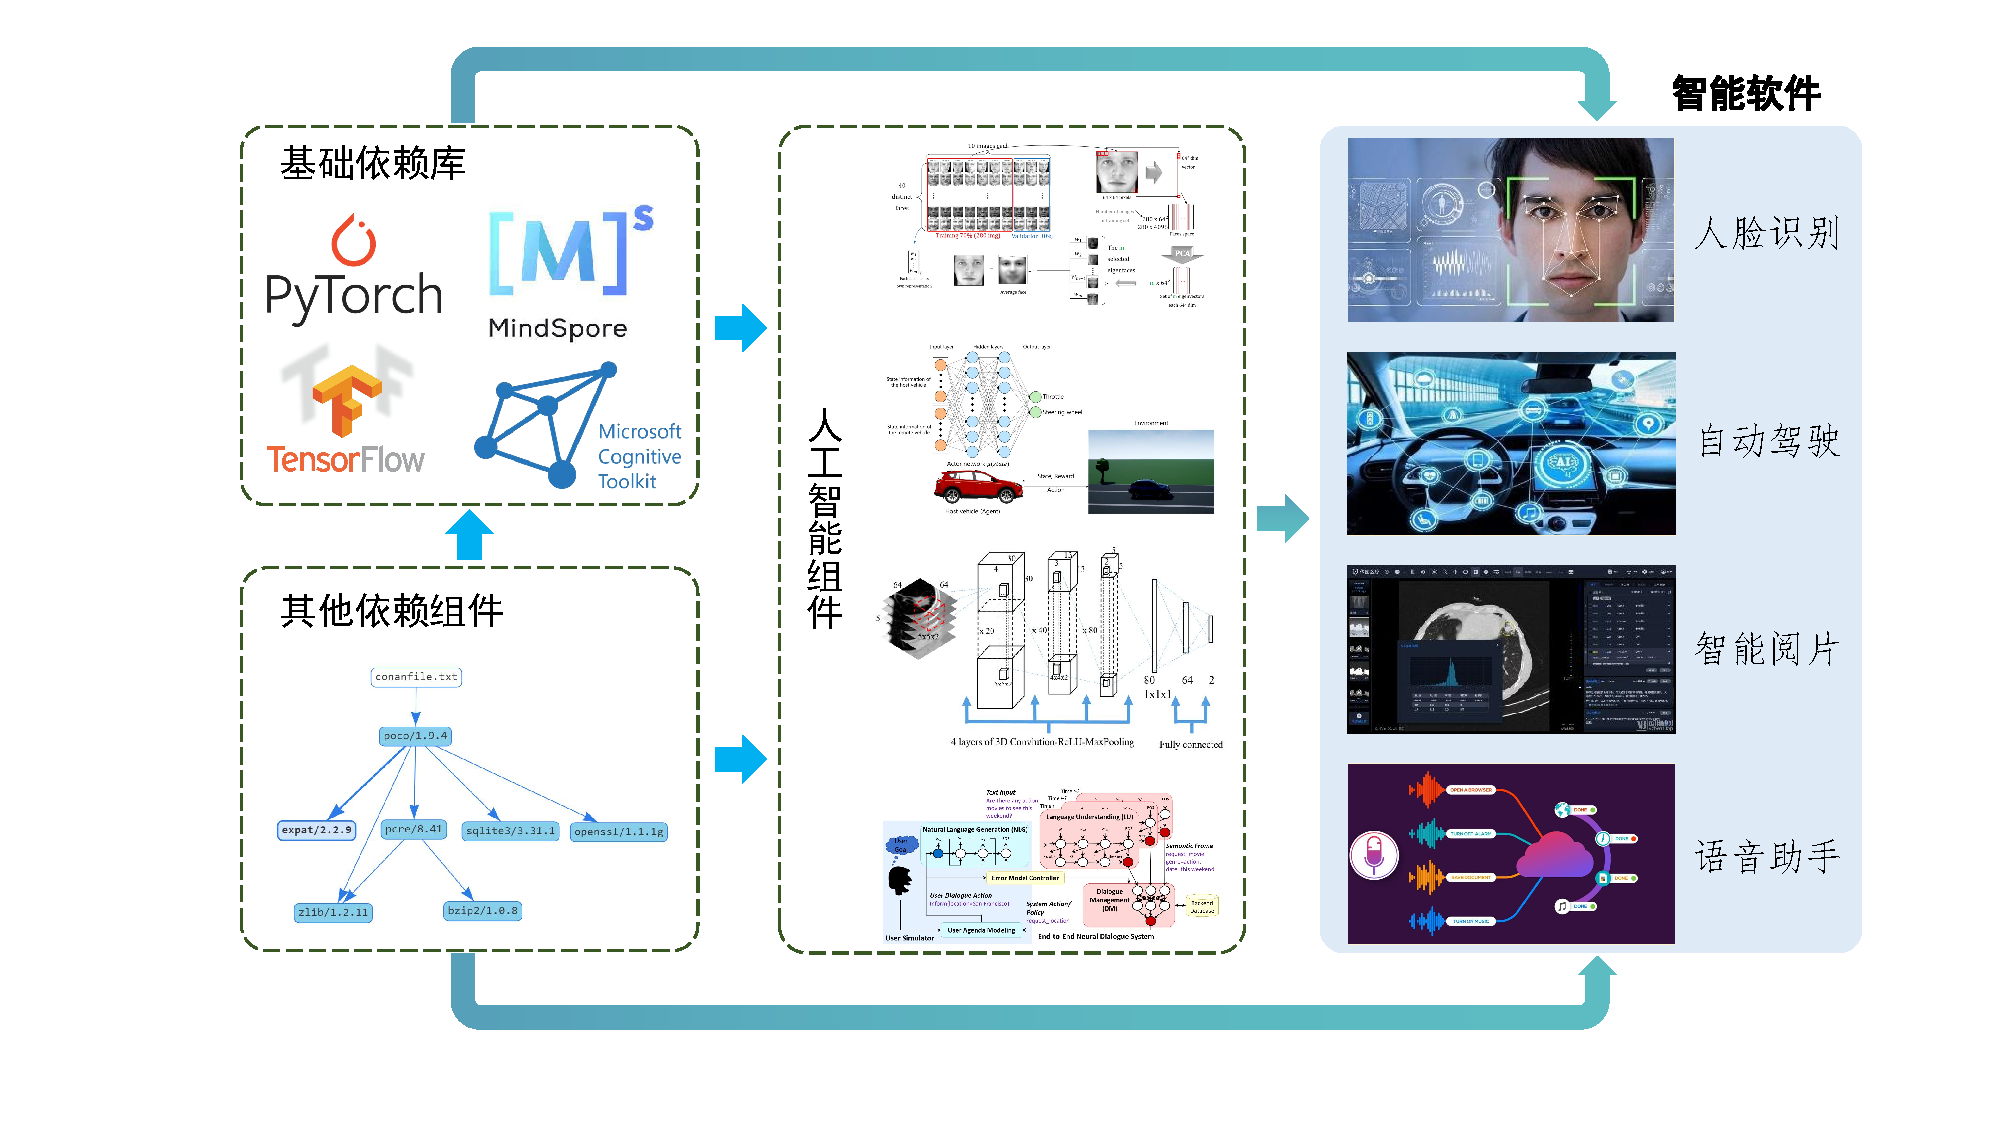
\includegraphics[width=0.9\linewidth]{Ch1AISoftware.pdf}
    \caption{智能软件依赖于多类型组件。}
    \label{fig:ch1:aisoftware}
\end{figure}

近年来,在人工智能技术获得巨大成功的同时,\textbf{对智能软件的安全性和可靠性的担
忧和关注也越来越多}。2018年3月,在美国亚利桑那州,一辆处在自动驾驶状态的Uber撞击
一名女子,致其不幸身亡,同年7月,Uber宣布停止研发自动驾驶货车。Szegedy等人首次发
现,数据中微小的扰动,即便无法被人类发现,却可能造成智能软件做出错误的判断,进而
输出错误的结果。由于智能软件越来越多地被部署在自动驾驶、恶意软件检测以及飞机碰撞
避免等安全攸关系统,因此迫切需要找到这些潜在的威胁来提高智能软件的安全性,使之能
够应用于更多关键任务场景。\textbf{本项目申请人也在自动驾驶软件安全方面提出了针对
神经网络模型的确定性测试数据集生成方法}。

%2019年国家新一代人工智能治理专业委员会发布《新一代人工智能治理原则——发展负责任的人工智能》,该文件中指出“\textbf{人工智能系统应不断提升透明性、可解释性、可靠性、可控性},逐步实现可审核、可监督、可追溯、可信赖”。

% 2. 现有工作和方法的不足
为了提高智能软件的安全性和可靠性,目前国内外许多关于人工智能鲁棒性和确定性的研
究,包括对抗攻击、中毒攻击、结构推理、层次化分析等。在智能软件测试方面,加拿大阿
尔伯塔大学的Lei Ma团队在覆盖性指标、测试数据生成、鲁棒性和模型修复等方面展开了深
入研究。国内南京大学的陈振宇老师团队在对话系统、医疗、自动驾驶、机器翻译、司法文
书等领域展开智能软件测试方法研究。然而,\textbf{现有工作主要集中于单个智能组件的
脆弱性,关于基础库和第三方组件的漏洞研究较少,尤其忽略了第三方组件漏洞对智能组件
的影响}。如\cref{fig:ch1:target}所示,。。。\textbf{可见,第三方开源组件中存在
的漏洞也可以作为攻击智能组件脆弱点的突破口,从而威胁整个智能软件的安全性和可靠
性}。
\begin{figure}[htp]
    \centering
    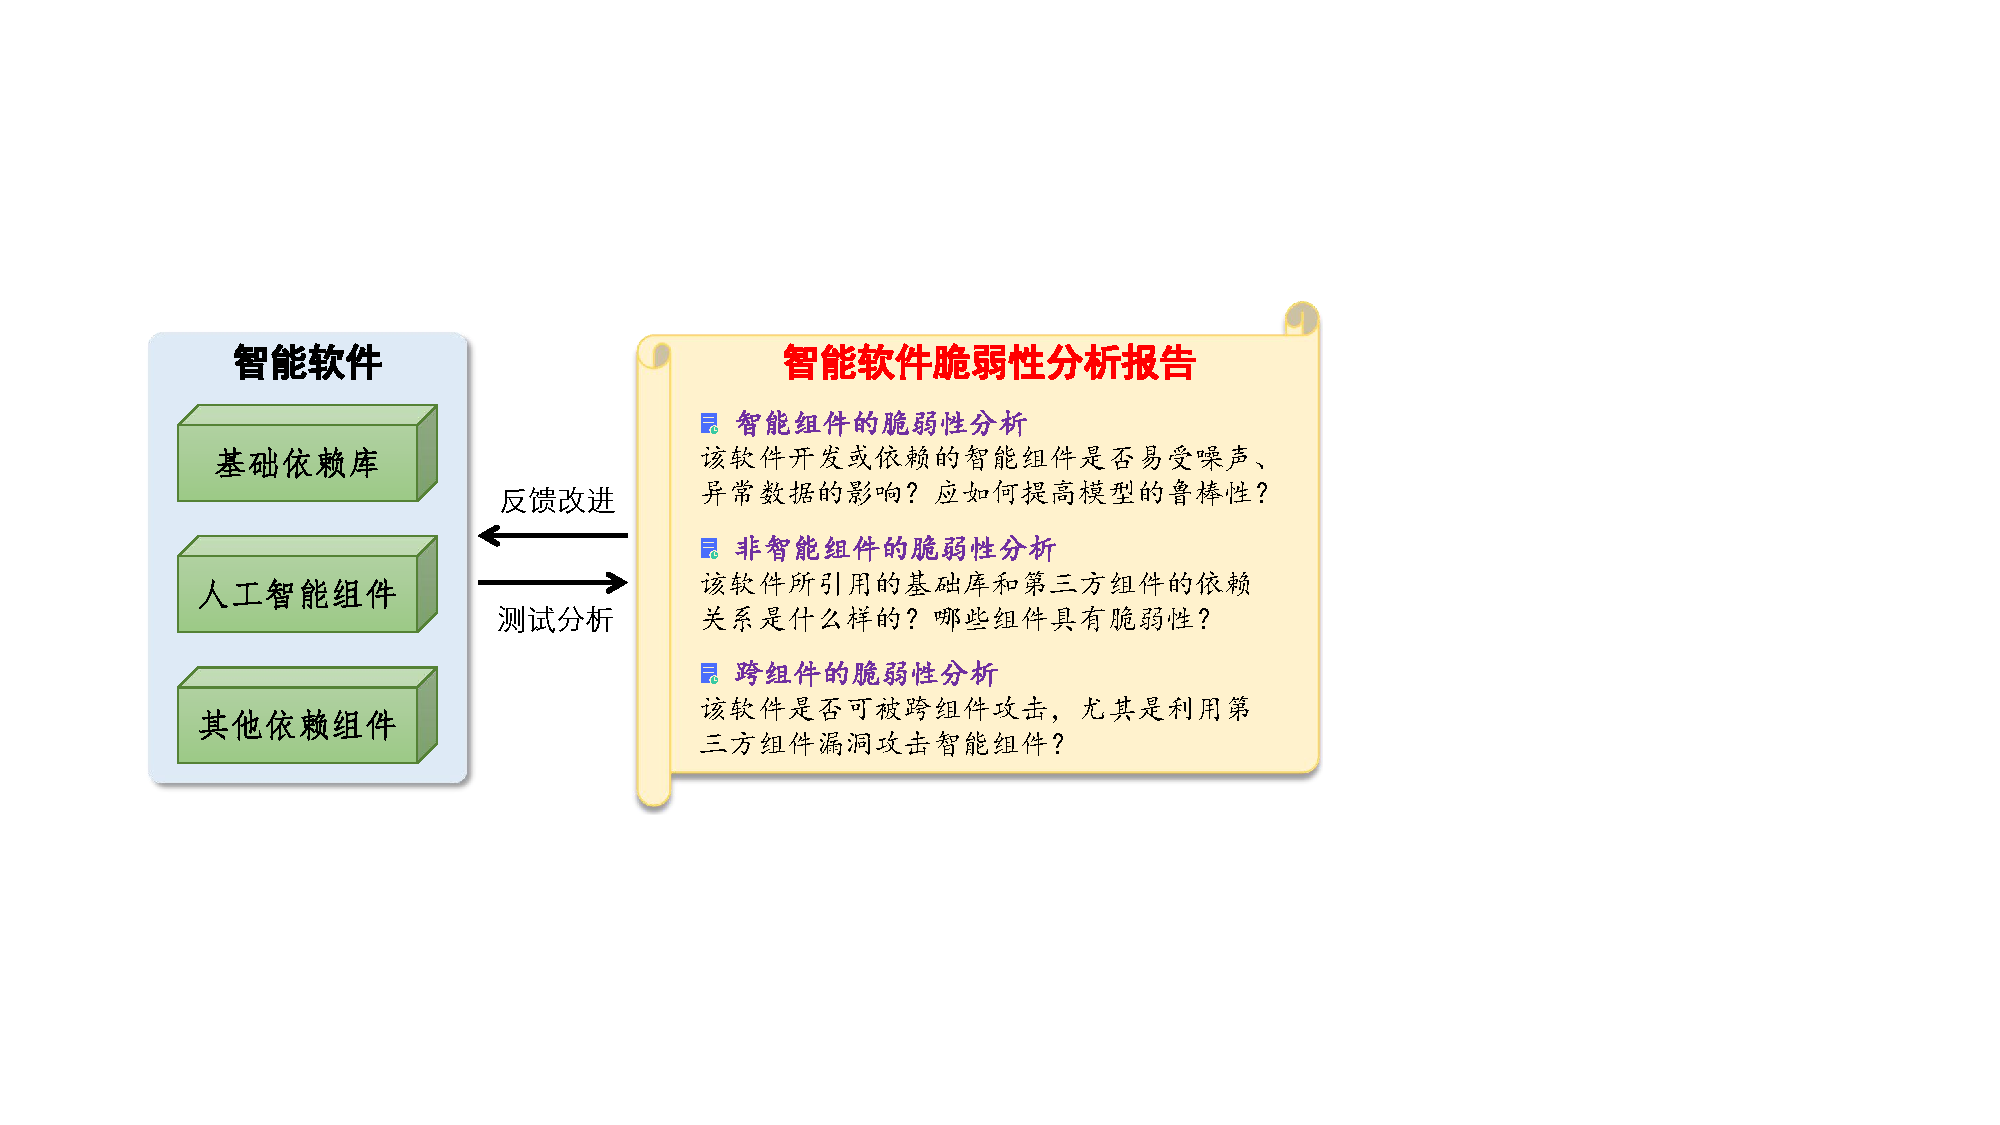
\includegraphics[width=0.9\linewidth]{Ch1ProjectTarget.pdf}
    \caption{智能软件依赖于多类型组件。}
    \label{fig:ch1:target}
\end{figure}

% 3. 研究挑战
结合智能软件的特点和安全可靠的应用需求,智能软件脆弱性分析具有以下挑战:

\begin{itemize}
    \item[(1)]\textbf{不确定性}:智能组件本身的不确定性导致其易受噪声和异常样本攻击,做出错误预测。
    \item[(2)]\textbf{复杂性}:智能软件开发基础库和第三方库庞大,难以筛选脆弱组件,找到组件漏洞。
    \item[(3)]\textbf{高隐蔽性}:利用第三方组件漏洞攻击智能软件不易被发现。
\end{itemize}





% 4. 研究方法
% 5. 研究意义



\subsection{国内外研究现状及发展动态分析}\label{relatedwork}

根据与本项目的相关性,本节从电子医疗记录的表示学习、表现型分析、数据插补、以及模
型的可解释性四个方面介绍和分析国内外研究现状。

%(1) 电子医疗记录表示学习\textbf{}
\subsubsection{电子医疗记录表示学习}

电子医疗记录的表示学习借鉴于自然语言处理领域的词嵌入(word embedding),尤其是
word2vec~\citess{mikolov2013efficient,mikolov2013distributed}模型。表示学习的基
本思想是:出现在相似上下文的特征具有相似的语义信息,即相似的向量表示。好的医疗特
征表示能合理地反映医疗特征之间的语义关系,有助于电子医疗记录的分析。

基于电子医疗记录的表示学习研究工作如\cref{tab:representation}所示。Tran等人~\citess{tran2015learning}利用非负玻尔兹曼机(Nonnegative Restricted Boltzman
Machine)学习医学特征的向量表示,是最早使用深度学习的研究方法;Miotto等人~\citess{miotto2016deep}和Choi等人~\citess{choi2016medical}也较早的利用其他深度
学习模型学习学习医疗特征的表示;\textbf{本项目申请人蔡祥睿~\citess{cai2018medical}首先提出不同医疗特征的时间作用域有差别,其上下文界定不能
设置为固定超参数,并引入注意力机制,学习医疗特征不同的上下文时间范围};Peng等人~\citess{peng2019temporal}在此基础上设计更复杂的注意力模型,进一步提高特征表示学
习的效果。这些工作所使用的数据只有电子医疗记录数据集;Bai等人~\citess{bai2019medical}提出对齐多医疗机构的特征并学习其表示。Choi等人~\citess{choi2017gram,choi2018mime}率先在医疗特征表示学习模型中引入领域知识;Ma
等人~\citess{ma2018kame}也提出了相似的思路,并将所学特征表示用于疾病诊断的预测;
Song等人~\citess{song2019medical}面向多个机构的电子医疗记录表示学习,通过引入了
医学领域的知识库进行语义对齐。部分研究工作通过结合电子医疗记录、病历和文献等异构
数据进行模型训练,期望得到更好的特征表示~\citess{choi2016learning,bai2017joint,ma2018drug}. 此外,Choi等人还提出了针对医
疗特征和患者就诊两个层次的表示学习模型~\citess{choi2016multi},以及利用图神经网
络学习医疗特征之间的关联关系~\citess{choi2020learning},这些工作在医疗特征表示学
习中引入了数据的结构知识。

\begin{table}
    \renewcommand\arraystretch{1.5}
    \begin{small}
        \caption{EMR表示学习相关研究工作}
        \label{tab:representation}
        \begin{center}
            \begin{tabular}[c]{cll}
                \toprule
                \multicolumn{1}{c}{\textbf{序号}} &
                \multicolumn{1}{c}{\textbf{主要思想}} &
                \multicolumn{1}{c}{\textbf{文献号}}\\
                \midrule
                1 & 仅基于EMR数据集训练医疗特征表示 & \cite{tran2015learning}
                \cite{miotto2016deep} \cite{choi2016medical}
                 \cite{cai2018medical} \cite{peng2019temporal}
                 \cite{bai2019medical}\\
                2 & 结合EMR数据集和医疗领域知识库 & \cite{choi2017gram}
                \cite{choi2018mime} \cite{ma2018kame} \cite{song2019medical}\\
                3 & 基于异构医疗数据学习医疗特征表示 & \cite{choi2016learning}
                \cite{bai2017joint} \cite{ma2018drug}\\
                4 & 学习层次化的EMR数据表示 & \cite{choi2016multi}
                \cite{choi2020learning}\\
                \bottomrule
            \end{tabular}
        \end{center}
    \end{small}
\end{table}

{\kaishu{电子医疗记录中特征表示与表现型直接相关,是队列识别的重要研究问题之一,
特征表示是表现型表示和队列识别的基础。现有工作主要聚焦于针对医疗特征的向量表示学
习研究,缺少对高层次语义表示的研究,如表现型表示。本课题拟引入表现型向量字典,将
患者表示为多个高层次表现型的组合,从而提升队列识别的准确率。}}

\subsubsection{电子医疗记录表现型分析}

表现型是一组患者或者疾病的属性,根据表现型不同可以将患者划分成更有意义的分组,与
本项目研究内容队列识别直接相关。面向电子医疗记录的表现型分析的主要方法如
\cref{tab:phenotype}所示。

针对电子医疗记录进行表现型分析的人物最早由现在UIUC的Jimeng Sun教授团队引入计算机
领域,他们将电子医疗记录看作张量,利用张量分解进行降维分析~\citess{ho2014extracting},随后,该团队还先后将基于张量分解的模型扩展到联邦学习~\citess{kim2017federated}和无监督学习~\citess{perros2018sustain}的场景中,由于
电子医疗记录的高维性,张量分解的效率较低,Heano等人~\citess{heano2018parallel}和
He等人~\citess{he2019distributed}研究如何利用并行和分布式技术进行加速。基于张量
分解的模型缺乏对记录时间的考虑,部分研究工作将电子医疗记录建模成图,图中的点为医
疗特征,特征记录如果相邻,则给图增加一条对应的边,边的权重与记录时间间隔相关,最
后利用图算法分析患者的表现型,如图分解~\citess{liu2015temporal}、频繁子图挖掘~\citess{wang2015graph,xu2017predicting}等方法。深度学习模型擅长表示学习,非常适
合表现型分析,同时,挖掘表现型也能提高深度学习模型的可解释性~\citess{kale2015causal}。Che等人~\citess{che2015deep}较早的将医疗编码的层次结构
引入基于深度学习的表现型分析模型;Beaulieu-Jones等人~\citess{beaulieu2016semi}提
出基于去噪自编码器的半监督模型,不需要大量标注样本,是本项目的重要参考;Baytas等
人~\citess{baytas2017patient}利用表现型对患者进行细粒度的划分;Fu等人~\citess{fu2019ddl}首次提出面向表现型的深度字典学习,为本项目引入表现型字典提供
了理论依据;Seymour等人~\citess{seymour2019derivation}利用深度学习研究感染性休克
的表现型,是本项目研究感染性休克预测的重要参考。

\begin{table}
    \renewcommand\arraystretch{1.5}
    \begin{small}
        \caption{针对EMR的表现型分析方法}
        \label{tab:phenotype}
        \begin{center}
            \begin{tabular}[c]{cll}
                \toprule
                \multicolumn{1}{c}{\textbf{序号}} &
                \multicolumn{1}{c}{\textbf{主要思想}} &
                \multicolumn{1}{c}{\textbf{文献号}}\\
                \midrule
                1 & 以张量表示EMR数据集,进行张量分解 &
                \cite{ho2014extracting} \cite{kim2017federated}
                \cite{perros2018sustain} \cite{heano2018parallel} \cite{he2019distributed}
                \cite{perros2019temporal} \\
                2 & 将EMR建模成图,利用图算法分析表现型 & \cite{liu2015temporal}
                \cite{wang2015graph} \cite{xu2017predicting} \\
                3 & 基于深度学习模型,多为监督学习 & \cite{kale2015causal}
                \cite{che2015deep}
                \cite{beaulieu2016semi} \cite{cheng2016risk}
                \cite{baytas2017patient} \cite{fu2019ddl} \cite{seymour2019derivation} \\
               \bottomrule
            \end{tabular}
        \end{center}
    \end{small}
\end{table}

{\kaishu {现有基于深度学习的表现型分析模型绝大多数都是有监督模型,需要大量的标注
样本,难以在真实医疗场景中应用。值得注意的是,部分研究工作直接基于医疗特征表示进
行队列识别,如~\cite{glicksberg2018automated,bai2018ehr},由于电子医疗记录的高维
性,这类方法容易得到相似度较高的患者表示,不利于队列识别。}}

\subsubsection{电子医疗记录插补}

因为患者就医时间没有规律,电子医疗记录呈现时间不规则性,直接利用现有模型分析电子
医疗记录难以取得较好的结果,因此,数据插补对电子医疗记录的分析具有重要意义。关于
电子医疗记录插补的相关工作总结如\cref{tab:imputation}所示。

针对数据缺失值的插补很早就被关注,最传统的方式是利用均值、中位数进行插补,但缺乏
对数据分布的考虑,效果较差。基于传统机器学习模型进行插补近年来也一直有研究者在关
注,Beaulieu-Jones等人~\citess{beaulieu2018characterizing}在电子医疗记录上对比了
12中传统机器学习模型方法,发现MICE~\citess{sterne2009multiple}很多情况下能取得较
好的结果。值得注意的是,Zheng等人~\citess{zheng2017resolving}较早的提出了要考虑
电子医疗记录中的医学偏差,并利用隐马尔可夫模型加入对偏差的考虑,但该工作只推断患
者的状态,不能得到缺失值的插补。随着深度学习的发展,越来越多的研究工作开始利用深
度学习模型处理电子医疗记录中的缺失值,Che等人~\citess{che2018recurrent}较早地利
用RNN模型进行电子医疗记录插补,为考虑时间不规则性的影响,他们设计了时间衰减因
子,Cao等人~\citess{cao2018brits}和Suo等人~\citess{suo2019recurrent}构建更复杂的
RNN模型,进一步提升\cite{che2018recurrent}的效果。除了RNN模型,少量研究工作也以
AutoEncoder为主干模型,实现电子医疗记录插补~\citess{beaulieu2017missing,costa2018missing}。\textbf{最近,本项目申请人首先提
出将插补问题看成数据生成问题,并构建基于生成对抗网络(Generative Adversarial
Network,GAN)的数据插补模型~\citess{luo2018multivariate,luo20192},在该领域取得
了国际领先结果}。此外,Yoon等人~\citess{yoon2018gain}同样利用GAN进行数据插补,
Mattei等人~\citess{mattei2019miwae}首次在本问题上采用深度隐变量模型(Deep Latent
Variable Model),但它们的数据假设局限于完全随机缺失(Missing Completely At
Random)和非时序数据,无法应用于电子医疗记录。

\begin{table}
    \renewcommand\arraystretch{1.5}
    \begin{small}
        \caption{EMR插补相关研究工作}
        \label{tab:imputation}
        \begin{center}
            \begin{tabular}[c]{cll}
                \toprule
                \multicolumn{1}{c}{\textbf{序号}} &
                \multicolumn{1}{c}{\textbf{主要思想}} &
                \multicolumn{1}{c}{\textbf{文献号}}\\
                \midrule
                1 & 传统机器学习模型 & \cite{zheng2017resolving}
                \cite{beaulieu2018characterizing} \cite{yang2018time} \cite{xu2019estimating} \cite{sterne2009multiple}
                \\
                2 & 基于RNN的缺失值预测模型 &
                \cite{che2018recurrent} \cite{suo2019recurrent}
                ~\cite{cao2018brits} \\
                3 & 基于AutoEncoder模型重构缺失值 & \cite{beaulieu2017missing}
                \cite{costa2018missing} \\
                4 & 基于生成模型进行缺失值生成 & \cite{luo2018multivariate}
                \cite{luo20192} \cite{yoon2018gain} \cite{mattei2019miwae} \\
               \bottomrule
            \end{tabular}
        \end{center}
    \end{small}
\end{table}

电子医疗记录中的偏差是医学领域中的常见问题,已经被许多医学研究证实:Pivovarovd等
人~\citess{pivovarov2014identifying}利用特征出现的频率识别临床检测数据中的偏差,
Phelen等人~\citess{phelan2017illustrating}举例说明了电子医疗记录中医学偏差产生的
原因,Agniel等人~\citess{agniel2018biases}设计回顾性分析实验,证明了医学偏差在电
子医疗记录中普遍存在,Vassy等人~\citess{vassy2018yield}利用可视化分析发现偏差。
这些研究结果指出,医学偏差可以作为一种特征,有助于理解数据。

{\kaishu{本项目拟将医学偏差作为患者分布的特征,通过将其引入电子医疗记录插补模
型,实现隐式地进行细粒度患者划分,提高数据插补的准确性。目前已有研究可以佐证引入
医学偏差能提高模型效果,但尚未有相关研究在基于深度学习的插补模型中引入医学偏差,
本项目的研究正好补充该方向上的空白。}}

\subsubsection{模型可解释性}

拥有良好的可解释性是机器学习模型实际应用的重要保证,这在医疗数据分析领域尤其重
要。虽然目前越来越多的研究工作开始利用深度学习对电子医疗记录建模,但可解释性是深
度学习的基础性难题,尚无非常完备的解决的方案。\cref{tab:interpretability}总结了
电子医疗记录分析模型可解释性的研究。现有关于电子医疗记录分析的可解释性研究主要分
为两类:1)将模型看作黑盒(black-box),待模型训练完以后再对分析结果进行解释
(Post-hoc);2)改进模型,使模型本身具有可解释性(Ante-hoc)。除了这两类模型方
面的研究以外,也有一些工作研究可视化交互界面,建立人机互动的平台。

\begin{table}
    \renewcommand\arraystretch{1.5}
    \begin{small}
        \caption{EMR模型可解释性相关研究工作}
        \label{tab:interpretability}
        \begin{center}
            \begin{tabular}[c]{cll}
                \toprule
                \multicolumn{1}{c}{\textbf{序号}} &
                \multicolumn{1}{c}{\textbf{主要思想}} &
                \multicolumn{1}{c}{\textbf{文献号}}\\
                \midrule
                1 & 将模型看作黑盒,对预测结果进行解释(Post-hoc) & \cite{panigutti2019explaining}
                \cite{panigutti2020doctor} \\
                2 & 修改模型结构,在预测同时提供可解释性(Ante-hoc) &
                \cite{choi2016retain} \cite{ma2017dipole} \cite{bai2018interpretable}
                \cite{gao2019camp} \cite{ma2019adacare} \\
                3 & 利用可视化界面,便于理解 & \cite{kwon2018retainvis} \cite{jin2020carepre}
                \cite{guo2020comparative} \\
                \bottomrule
            \end{tabular}
        \end{center}
    \end{small}
\end{table}

LIME~\citess{ribeiro2016should}最早提出将模型看作黑盒,并逐样本解释预测结果的方
法;Panigutti等人~\citess{panigutti2019explaining}首先利用这种方法解释电子医疗记
录分析模型,但该工作解释的模型缺少时间属性;随后,他们由针对考虑时间的模型应用相
同的思想,提出了Doctor XAI~\citess{panigutti2020doctor}。这类方法的核心思想是利
用给定样本周边的样本训练一个简单模型,以此对原模型预测的可靠性做出解释,方法无法
给出原模型决策的原因。我们知道,对抗样本仅对原样本做了一点微小的改变,却能改变模
型预测结果~\citess{su2019one},因此Post-hoc的方法难以在医疗领域广泛应用。

Ante-hoc方法主要是通过注意力机制对模型进行改造,使其具有可解释性。
Choi~\citess{choi2016retain}于2016年提出RETAIN模型,将RNN隐含层的部分计算转移给
注意力机制,虽然一定程度上提高了模型可解释性,但其预测准确率较低;Bai等人~\citess{bai2018interpretable}和Ma等人~\citess{ma2019adacare}分别提出了针对
RETAIN模型的改进。Dipole模型~\citess{ma2017dipole}只能提供关于预测目标比较的重要
就医记录(一次就医的所有记录),无法进一步细粒度分析。这些模型仅考虑了动态特征,
忽略了静态特征的影响。Gao等人~\citess{gao2019camp}虽然同时考虑了静态特征和动态特
征,但两组特征的重要性是分别计算的,没有得到全局下的特征权重,而且该模型无法总结
出模型的行为准则,每个病历需要单独判别。

在可视化医疗分析平台方面,Kwon等人~\citess{kwon2018retainvis}为RETAIN做了可视化
界面;Jin等人~\citess{jin2020carepre}提出了交互式的智能医疗决策辅助平台CarePre;
而Guo等人~\citess{guo2020comparative}聚焦于可视化电子医疗记录,为基于不同队列的
对比研究提供辅助。这些可视化分析方法和平台,是本项目系统研发的重要参考。



{\kaishu{现有可解释性研究无法对模型的预测行为进行全局分析,本项目拟提出可溯源的
电子医疗记录分析模型,通过同时比较静态特征和动态特征对预测结果的贡献,可从整体上
分析特征的变化对模型的影响。此外,本项目拟研发可视化界面呈现模型可解释分析结
果。}}

% 因为写 demo,我把参考文献放这里了,真写本子的时候,还是要放在国内外概况那边
\begin{spacing}{1.3} % 行距
	\zihao{5} \songti
	\bibliographystyle{gbt7714-nsfc}
	\bibliography{ref}
	\vspace{11bp}
\end{spacing}
